\documentclass[a4paper,notitlepage,12pt]{report}
\usepackage[utf8]{inputenc}
\usepackage[T1]{fontenc}
\usepackage[german]{babel}
\usepackage[margin=2cm]{geometry}
\usepackage{url}
\usepackage{graphicx}
\usepackage{tikz}
\usepackage{subcaption}
\usepackage{float}
\usepackage[bottom]{footmisc}
\usepackage{titling}
\usepackage{nomencl}
\usepackage{titlesec}
\usepackage{pgfplots}

\renewcommand{\nomname}{\Huge \textbf{Abkürzungsverzeichnis}}
\makenomenclature
\nomenclature{TSP}{Traveling Salesman Problem}
\nomenclature{VRP}{Vehicle Routing Problem}
\nomenclature{OSRM}{Open Source Routing Machine}
\nomenclature{VO}{Visual Objects}

\pretitle{\begin{center}\Huge}
\posttitle{\par\end{center}\vskip 0.5em}
\preauthor{\begin{center}\Large}
\postauthor{\end{center}}
\predate{\par\large\centering}
\postdate{\par\vskip 5em}

\titleformat{\chapter}[display]
{\normalfont\huge\bfseries}{}{0pt}{\Huge}

\titlespacing*{\chapter}
{0pt}{10pt}{40pt}

\title{Automatische Einsatzplanung \\
    \large Lösung eines VRP mithilfe eines Evolutionäreren Algorithmus}
\author{Roland Bernard}
\date{2020-05-10}

\begin{document}
\maketitle
\begin{abstract}

    Ziel dieses Projektes war es eine Software zu entwickeln, welche es 
    ermöglicht Einsätze automatisch und so effizient wie möglich zu Planen.
    Zur Umsetzung dieses Zieles wurde ein Evolutionärer Algorithmus verwendet.
    Ein solcher Algorithmus lehnt sich an die biologische Evolution an und
    kann so das Problem relativ erfolgreich lösen.

\end{abstract}
\newpage

\addcontentsline{toc}{chapter}{Inhaltsverzeichnis}
\tableofcontents
\newpage
\addcontentsline{toc}{chapter}{Abbildungsverzeichnis}
\listoffigures
\newpage
\addcontentsline{toc}{chapter}{Tabellenverzeichnis}
\listoftables
\newpage
\addcontentsline{toc}{chapter}{Abkürzungsverzeichnis}
\printnomenclature
\newpage

\chapter{Einleitung}

\section{Überblick}

Die Aufgabe, die es zu lösen gilt, ist es anstehenden Serviceeinsätze auf sein
Team von Technikern möglichst effizient zu verteilen. Die Aufgabe besteht
darin, für diese Aufgabe einen Algorithmus zu entwickeln, der eine automatische
Zuteilung der Techniker vornimmt. Der Algorithmus soll die anstehenden Einsätze
auf die Techniker so verteilen, dass die Fahrtzeiten so gering wie möglich ausfällt
und die Einsätze aufgrund ihrer Priorität so zeitnah als möglich eingeplant werden.

\section{Die Motivation}

Das Problem wurde von der Firma Infominds vorgeschlagen. Infominds entwickelt eine
Business Software mit dem Namen RADIX \cite{radix}, welche das Eintragen, Anzeigen und Analysieren
von Geschäftsdaten und Geschäftsprozessen ermöglicht. In dieser Software werden
ist auch ein Ticketsystem integriert, für welches eine solche Einsatzplanung
hilfreich wäre. Mit der Einsatzplanung könnte das Personal, welches momentan noch
manuell alle Routen plant unterstützt werden.

\section{Problemdefinition}

Gegeben ist eine Liste an Technikern und eine Liste an Einsätzen.

\begin{itemize}
    \item
    Für jeden Techniker
    \begin{itemize}
        \item Start-/Endposition (Die Techniker kehren wieder an ihre Ausgangsposition zurück.)
        \item Arbeitszeit, die der Techniker maximal arbeitet
    \end{itemize}
    \item
    Für jeden Einsatz
    \begin{itemize}
        \item Position des Einsatzes
        \item Dauer des Einsatzes (Diese muss geschätzt werden, um die Arbeitszeiten einzuhalten.)
        \item Priorität des Einsatzes (Das genaue Format ist nicht festgelegt.)
    \end{itemize}
\end{itemize}

Zu minimieren sind dabei die benötigten Fahrzeiten der Techniker. Dabei zu
berücksichtigen ist sowohl die Arbeitszeit der einzelnen Techniker, diese darf
nämlich nicht überschritten werden, als auch die Priorität der Einsätze. Um
diese weiteren Aspekte zu berücksichtigen, sollte ebenfalls die nach Priorität
gewichtete Wartezeit der Einsätze minimiert werden.

\section{Stand der Technik}

Dieses Problem ähnelt bereits bekannten Problem in der Informatik wie dem TSP \cite{tsp} oder
dem VRP \cite{vrp}. Es handelt sich hierbei zwar um eine Art VRP, aber beide diese Probleme
sind meist weniger komplex als das hier gegebene und
die Lösungen, die für diese angewandt werden, können nicht einfach übertragen werden.
Auch sind sowohl TSP und VRP als auch das Problem der Einsatzplanung NP-Hard. Das
bedeutet also, das es keinen effizienten Algorithmus gibt, der die genaue Lösung
des Problems finden kann. Man muss sich also mit Heuristiken behilflich sein, welche
nur eine gute aber nicht unbedingt die beste Lösung zurückliefern.

\section{Beispiel}

\begin{figure}[H]
    \begin{center}
        \begin{tikzpicture}
            \draw [] (-1, -1) rectangle (10, 10);
            \draw [fill] (1, 5) rectangle (0.6, 4.6) node [black,below] {Techniker 1};
            \draw [fill] (8, 6) rectangle (7.6, 5.6) node [black,below] {Techniker 2};
            \draw [fill] (9, 1) rectangle (8.6, 0.6) node [black,below] {Techniker 3};
            \draw [yellow,fill] (3, 7) circle [radius=0.2] node [black, below] {Einsatz 1};
            \draw [yellow,fill] (4, 9) circle [radius=0.2] node [black, below] {Einsatz 2};
            \draw [red,fill] (3.5, 3) circle [radius=0.2] node [black, below] {Einsatz 3};
            \draw [yellow,fill] (5, 2) circle [radius=0.2] node [black, below] {Einsatz 4};
            \draw [yellow,fill] (7, 1) circle [radius=0.2] node [black, below] {Einsatz 5};
        \end{tikzpicture}
        \caption{Beispiel für ein mögliche Problemstellung}
    \end{center}
\end{figure}

Die Kreise seien die Ausgangspositionen der Techniker und die Rauten die Positionen
der Einsätze. Für das Beispiel nehmen wir an, dass die Abstände zwischen den Einsätzen
proportional zu den Fahrzeiten sind. Diese Annahme macht das Problem, wie sich
herausstellt, nämlich nicht einfacher.

Im oben stehenden Beispiel wäre die Lösung, welche die geringste Fahrzeit in Anspruch
nimmt, die bei welcher Techniker 1 Einsatz 1 und Einsatz 2 übernimmt und Techniker 3
die restlichen drei Einsätze.

\begin{figure}[H]
    \begin{center}
        \begin{subfigure}[b]{0.45\linewidth}
            \begin{tikzpicture}
                \draw [] (-0.5, -0.5) rectangle (5, 5);

                \draw [thick] (0.4, 2.4) to (1.5, 3.5);
                \draw [thick] (1.5, 3.5) to (2, 4.5);
                \draw [thick] (0.4, 2.4) to (2, 4.5);

                \draw [thick] (4.4, 0.4) to (1.75, 1.5);
                \draw [thick] (1.75, 1.5) to (2.5, 1);
                \draw [thick] (3.5, 0.5) to (2.5, 1);
                \draw [thick] (4.4, 0.4) to (3.5, 0.5);

                \draw [fill] (0.5, 2.5) rectangle (0.3, 2.3) node [black,below] {};
                \draw [fill] (4, 3) rectangle (3.8, 2.8) node [black,below] {};
                \draw [fill] (4.5, 0.5) rectangle (4.3, 0.3) node [black,below] {};

                \draw [yellow,fill] (1.5, 3.5) circle [radius=0.1] node [black, below] {};
                \draw [yellow,fill] (2, 4.5) circle [radius=0.1] node [black, below] {};
                \draw [red,fill] (1.75, 1.5) circle [radius=0.1] node [black, below] {};
                \draw [yellow,fill] (2.5, 1) circle [radius=0.1] node [black, below] {};
                \draw [yellow,fill] (3.5, 0.5) circle [radius=0.1] node [black, below] {};
            \end{tikzpicture}
            \caption{Beste Lösung für die Problemstellung ohne maximale Arbeitszeit und Priorität}
        \end{subfigure}
        \begin{subfigure}[b]{0.45\linewidth}
            \begin{tikzpicture}
                \draw [] (-0.5, -0.5) rectangle (5, 5);

                \draw [] (-0.5, -0.5) rectangle (5, 5);

                \draw [thick] (0.4, 2.4) to (1.5, 3.5);
                \draw [thick] (1.5, 3.5) to (2, 4.5);
                \draw [thick] (0.4, 2.4) to (2, 4.5);

                \draw [thick] (4, 3) to (3, 2) to (1.75, 1.5);
                \draw [thick] (4, 3) to (2.75, 2.4) to (1.75, 1.5);

                \draw [thick] (4.4, 0.4) to (3.5, 0.5);
                \draw [thick] (3.5, 0.5) to (2.5, 1);
                \draw [thick] (4.4, 0.4) to (3.5, 0.85) to (2.5, 1);

                \draw [fill] (0.5, 2.5) rectangle (0.3, 2.3) node [black,below] {};
                \draw [fill] (4, 3) rectangle (3.8, 2.8) node [black,below] {};
                \draw [fill] (4.5, 0.5) rectangle (4.3, 0.3) node [black,below] {};

                \draw [yellow,fill] (1.5, 3.5) circle [radius=0.1] node [black, below] {};
                \draw [yellow,fill] (2, 4.5) circle [radius=0.1] node [black, below] {};
                \draw [red,fill] (1.75, 1.5) circle [radius=0.1] node [black, below] {};
                \draw [yellow,fill] (2.5, 1) circle [radius=0.1] node [black, below] {};
                \draw [yellow,fill] (3.5, 0.5) circle [radius=0.1] node [black, below] {};
            \end{tikzpicture}
            \caption{Beste Lösung für die Problemstellung ohne maximale Arbeitszeit und Priorität}
        \end{subfigure}
    \end{center}
    \caption{Beste Lösung für Teilproblemstellungen}
\end{figure}

Wenn wir nun aber annehmen, dass die Techniker 1 und 3 maximal zwei Einsätze am Tag
abarbeiten können, um die vorgegebene Arbeitszeit nicht zu überschreiten, so bedarf es
einer anderen Lösung. So ist die optimale Lösung nun Techniker 2 Einsatz 3 zu überlassen.


Betrachten wir nun aber auch die Priorität des Einsatzes, so könnte es sein, dass
der Einsatz 3 eine hohe Priorität hat, während alle anderen Einsätze eine sehr niedrige
Priorität haben. Dann wäre es wichtig den Einsatz 3 als Erstes abzuarbeiten. Techniker 1
hätte zudem die Möglichkeit schneller zu Einsatz 3 zu gelangen als Techniker 2. Die
optimale Lösung wäre demnach nun, dass Techniker 1 Einsatz 3 und Techniker 2 Einsatz 1
und 2 erledigt.

\begin{figure}[H]
    \begin{center}
        \begin{tikzpicture}
            \draw [] (-1, -1) rectangle (10, 10);

            \draw [thick] (0.8, 4.8) to (1.8, 3.8) to (3.5, 3);
            \draw [thick] (0.8, 4.8) to (2.2, 4.2) to (3.5, 3);

            \draw [thick] (7.8, 5.8) to (3, 7);
            \draw [thick] (3, 7) to (4, 9);
            \draw [thick] (7.8, 5.8) to (4, 9);

            \draw [thick] (8.8, 0.8) to (7, 1);
            \draw [thick] (7, 1) to (5, 2);
            \draw [thick] (8.8, 0.8) to (7, 1.75) to (5, 2);

            \draw [fill] (1, 5) rectangle (0.6, 4.6) node [black,below] {Techniker 1};
            \draw [fill] (8, 6) rectangle (7.6, 5.6) node [black,below] {Techniker 2};
            \draw [fill] (9, 1) rectangle (8.6, 0.6) node [black,below] {Techniker 3};

            \draw [yellow,fill] (3, 7) circle [radius=0.2] node [black, below] {Einsatz 1};
            \draw [yellow,fill] (4, 9) circle [radius=0.2] node [black, below] {Einsatz 2};
            \draw [red,fill] (3.5, 3) circle [radius=0.2] node [black, below] {Einsatz 3};
            \draw [yellow,fill] (5, 2) circle [radius=0.2] node [black, below] {Einsatz 4};
            \draw [yellow,fill] (7, 1) circle [radius=0.2] node [black, below] {Einsatz 5};
        \end{tikzpicture}
        \caption{Beste Lösung für die Problemstellung}
    \end{center}
\end{figure}

Das Beispiel soll aufzeigen, dass das zu lösende Problem keineswegs simpel ist und dass
das Finden einer Lösung durch die zusätzlichen Bedingungen, namentlich der maximalen
Arbeitszeit und der Priorität, erheblich erschwert wird.

\section{Das Ziel}

Das Ziel ist es einen Algorithmus auszuarbeiten und zu implementieren, der für eine
derartige Problemstellung eine gute Heuristik darstellt. Das Ergebnis sollte relativ
gut sein und die Ausführungszeit soll ebenfalls angemessen und nicht zu lang sein.
Der Algorithmus soll dann auch in die RADIX Software eingebunden werden können.

\chapter{Das Projekt}

\section{Projektanforderung}

Der entwickelte Algorithmus soll in verschiedenen Programmiersprachen relative
einfach zu implementieren sein, da er auch später in RADIX eingebaut werden soll.
Die Laufzeit des Algorithmus zum Erreichen einer guten Lösung für eine beliebige
Instanz des Problems soll relativ kurz sein. Es gibt keine spezielle Anforderung
an zu verwendende Technologien, da das ganze portabel gestaltet werden soll, um
es auch in anderen Programmiersprachen einfach umsetzen zu können.

\section{Voraussetzungen}

Dem Algorithmus, der das Problem lösen soll, müssen noch einige Daten zur
Verfügung gestellt werden. Und zwar die Fahrzeiten zwischen den verschiedenen
Einsätzen und Arbeitern. Zur Verfügung stehen nämlich nur die Adressen der
einzelnen Punkte und nicht deren Koordinaten oder die Fahrtzeiten zwischen ihnen.
Für dieses Problem gibt es aber bereits, anders als für das Hauptproblem, viele
einfache Lösungen. In den ersten beiden Test-Implementierungen wurde dafür das
Tool Nominatim \cite{nominatim} zur Auflösung der Positionen (Adresse zu Koordinaten) und dann
OSRM \cite{osrm} zur Berechnung der Fahrzeiten zwischen den Koordinaten verwendet. Diese
Projekte sind beide Open Source und sind vom Rest des Algorithmus unabhängig
und können deshalb beliebig ausgetauscht werden, falls der Wunsch besteht
andere Services zu nutzen. Bei der integrierung in die RADIX-Software zum
Beispiel wurden die bereits vorhandenen Koordinaten aus der Datenbank gelesen.

\section{Projektplanung}

\subsection{Algorithmus}

Zur Lösung des Problems kann eine Metaheuristik angewandt werden.
Also ein Algorithmus, der allgemein für Optimierungsalgorithmen
angewandt werden kann und nicht speziell für ein bestimmtes Problem erdacht
wurde. Dies erlaubt eine höhere Flexibilität und die Möglichkeit in der Zukunft
noch weitere Kriterien hinzuzufügen. Es gibt eine Vielzahl von Metaheuristiken,
aber aufgrund der hohen Komplexität des Problems scheint ein Evolutionärer
Algorithmus als die beste Wahl, da dieser damit generell sehr gut umgehen kann.

\subsubsection{Funktionsweise}

Ein Evolutionärer Algorithmus ist, wie der Name bereits verrät, an die biologische
Evolution angelehnt. Dabei gibt es eine sogenannte Population an Lösungen, welche
anfangs mit zufälligen Lösungen gefüllt wird. Dann wird über mehrere
Iterationen (Generationen) mithilfe von einer Funktion die Güte der Lösungen
ermittelt und die Lösungen werden zufällig miteinander vermischt (Crossover), dann
leicht verändert (Mutation) und in eine neue Population gegeben. Je höher die Güte
der Lösung ist, desto wahrscheinlicher ist es, dass die Lösung Teile von sich an
die nächste Population weitergibt. Durch wiederholte Iteration konvergiert die
Population dann in Richtung einer besseren Lösung. Gefährlich ist vor allem bei
komplexen Problemen, dass man in einem lokalen Minimum „gefangen“ bleiben kann.
Evolutionäre Algorithmen sind in dieser Hinsicht allerdings vorteilhafter als
andere Metaheuristiken.

\subsection{Repräsentation der Lösung}

Die Repräsentation der Lösung ist für die Qualität des Algorithmus sehr wichtig
und kann einen seh großen Einfluss darauf haben, wie schnell und auch wie gut die
Lösungen sind die gefunden werde, auch wenn zwei Repräsentationen immer das Gleiche
darstellen. Auch muss diese Repräsentation für die Operationen, die der Algorithmus
vornehmen muss, also Mutation und Crossover geeignet sein. Wie es auch bei
Implementierungen des TSP üblich ist, habe ich mich für eine Repräsentation als
Permutation entschieden. Eine mögliche Lösung wird also als Permutation mehrerer
Zahlen dargestellt. Dazu wird jedem Techniker und jedem Einsatz eine eindeutige
Zahl zugeordnet.

\begin{table}[H]
    \begin{center}
        \begin{tabular}{c|c|c|c|c|c|c|c|c|c}
            4 & 1 & 6 & 2 & 5 & 7 & 8 & 9 & 3 & 10
        \end{tabular}
    \end{center}
    \caption{Beispiel für eine mögliche Permutation als Lösung}
    \label{tab:exaSolPer}
\end{table}

In der Tabelle \ref{tab:exaSolPer} wird ein Beispiel für eine solche mögliche
Permutation dargestellt. In diesem Beispiel seien alle Zahlen von 0 bis 3 Techniker
und die übrigen Einsätze. Wie ihnen vielleicht auffällt, fehlt die Zahl 0. Diese
wird nämlich immer an erster Stelle angenommen, damit immer garantiert werden kann,
dass die Permutation eine mögliche Lösung repräsentiert. Alle Einsätze nach einem
Techniker und vor dem nächsten Techniker werden dann in der vorliegenden Reihenfolge
dem Techniker zugeordnet. Sollte die Abarbeitung der Einsätze mehrere Tage beanspruchen,
so wird der Pfad so weit hinten wie möglich geteilt.

\begin{table}[H]
    \begin{center}
        \begin{tabular}{c|cccccc}
            Techniker & \multicolumn{6}{c}{Einsätze} \\
            \hline
            0 & 4 & & & & & \\
            1 & 6 & & & & & \\
            2 & 5 & 7 & & & 8 & 9 \\
            3 & 10 & & & & &
        \end{tabular}
    \end{center}
    \caption{Beispiel für die Zuordung bei der gegebenen Permutation in der Tabelle \ref{tab:exaSolPer}}
    \label{tab:exaSolMea}
\end{table}

Wie angesprochen ist es wie im Beispiel beim Techniker 2 zu sehen möglich, dass die
Einsätze eines Technikers, falls notwendig, auf mehrere Pfade, also mehrere Tage,
aufgeteilt werden. Dadurch, dass die Trennung nur so möglich ist, gehen zwar einige
Lösungen verloren. Diese sind aber immer eher unerwünschte Lösungen, da sie erstens meist
längere Fahrzeiten in Anspruch nehmen und zweitens die Einsätze länger warten lassen
würden.

\subsection{Evaluierung einer Lösung}

Um die Qualität einer gegebenen Lösung zu bestimmen, muss eine sogenannte
Fitnessfunktion implementiert werden, welche einen höheren Wert ausgibt, wenn es
sich um eine gute Lösung handelt und eine niedrigeren wert errechnet, wenn es sich
um eine schlechtere Lösung handelt. Für diesen Zweck  wurde der Invers der Funktion
genommen, welche die Summe der Summe aller Fahrzeiten und der Summe aller
Wartezeiten gewichtet nach der Priorität der Einsätze errechnet. Es wurde deshalb
der Invers genommen, weil die Fitnessfunktion bei besseren Lösungen höher sein
muss als bei schlechteren und die Fahrzeit und Wartezeit natürlich besser ist,
wenn sie niedrig ist.
Diese Funktion berücksichtigt also die gesamte Fahrzeit, sowie die Priorität
der einzelnen Einsätze.

\subsection{Verbesserung der Lösungen}

\subsubsection{Mutation}

Für die Mutation wurden mehrere Funktionen gewählt, zwischen denen zufällig gewählt wird.
Die Mutationen die ich ausgewählt habe sind die folgenden.

\begin{itemize}
    \item Zwei Zahlen werden vertauscht. \\
        Zum Beispiel
        \begin{tabular}{c|c|c|c|c|c|c}
            1 & 2 & 3 & 4 & 5 & 6 & 7
        \end{tabular}
        zu
        \begin{tabular}{c|c|c|c|c|c|c}
            1 & 5 & 3 & 4 & 2 & 6 & 7
        \end{tabular},
        wenn die Elemente 2 und 5 vertauscht werden.
    \item Eine Zahl wird an eine neue Position verschoben. \\
        Zum Beispiel
        \begin{tabular}{c|c|c|c|c|c|c}
            1 & 2 & 3 & 4 & 5 & 6 & 7
        \end{tabular}
        zu
        \begin{tabular}{c|c|c|c|c|c|c}
            1 & 3 & 4 & 5 & 2 & 6 & 7
        \end{tabular},
        wenn das Elemente 2 an die Stelle 5 geschoben wird.
    \item Ein bestimmter Intervall wird umgekehrt. \\
        Zum Beispiel
        \begin{tabular}{c|c|c|c|c|c|c}
            1 & 2 & 3 & 4 & 5 & 6 & 7
        \end{tabular}
        zu
        \begin{tabular}{c|c|c|c|c|c|c}
            1 & 6 & 5 & 4 & 3 & 2 & 7
        \end{tabular},
        wenn der Interval von Elemente 2 bis Element 5 umgekehrt wird.
    \item Ein bestimmter Intervall wird an eine neue Position geschoben. \\
        Zum Beispiel
        \begin{tabular}{c|c|c|c|c|c|c}
            1 & 2 & 3 & 4 & 5 & 6 & 7
        \end{tabular}
        zu
        \begin{tabular}{c|c|c|c|c|c|c}
            1 & 6 & 2 & 3 & 4 & 5 & 7
        \end{tabular},
        wenn der Interval von Elemente 2 bis Element 5 an die Stelle 3 geschoben wird.
    \item Ein Intervall wird zufällig angeordnet. \\
        Zum Beispiel
        \begin{tabular}{c|c|c|c|c|c|c}
            1 & 2 & 3 & 4 & 5 & 6 & 7
        \end{tabular}
        zu
        \begin{tabular}{c|c|c|c|c|c|c}
            1 & 4 & 6 & 3 & 2 & 5 & 7
        \end{tabular},
        wenn der Interval von Elemente 2 bis Element 5 neu angeordnet wird.
\end{itemize}

Die Mutationsfunktionen müssen nicht besonders kompliziert sein, sondern nur dazu
dienen mehrere Variationen zu erschaffen. Dadurch wird vermieden, dass sich der
Algorithmus in einem lokalen Minimum festsetzt oder dass aufgrund von fehlender
Variation keine weiteren Verbesserungen möglich sind.

\subsubsection{Crossover}

Als Crossover-Funktion, also Funktion, welche zwei Lösungen kombiniert und daraus
eine neue Lösung generiert, welche Eigenschaften von beiden vorherigen Lösungen
hat, habe ich mehrere verschiedene Ansätze probiert. Darunter das Order 1-Crossover,
das Cycle-Crossover, das Edge-Rekombination-Crossover und das PMX-Crossover
ausprobiert. Am beste davon hat das PMX-Crossover abgeschnitten, da es eines der
schnellsten ist und generell gute Ergebnisse geliefert hat. Diese Crossover-Funktion
schlägt sich so gut, weil sie sowohl versucht die relativen Positionen als auch
die absoluten Positionen der einzelnen Elemente möglichst gut beizubehalten. Diese
Eigenschaften sind für ein Problem, bei dem sowohl die Zuordnung zu den Technikern
als auch die Reihenfolge der Abarbeitung wichtig ist, von Voreilt.

\section{Entwicklung}

\subsubsection{Python}

Den Algorithmus habe ich zuerst in der Programmiersprache Python programmiert um zu
testen ob dieser denn überhaupt funktioniert. Aufgrund dessen, dass Python aber
eine relativ langsame Programmiersprache ist, war diese Implementierung nicht
besonders schnell. Dennoch war dies genug um zu sehen, das die Implementierung
des Algorithmus möglich ist und der Algorithmus auch wie gewünscht funktioniert.

\subsubsection{RADIX}

Nach dieser ersten Implementierung habe ich den Algorithmus  in die RADIX-Software
integriert und ein dazugehöriges Benutzerinterface implementiert um die Nutzung
der existierenden Daten in der Datenbank zu benutzen. Diese Implementierung ist
in VO \cite{vo} implementiert, da dies die Programmiersprache ist in der RADIX geschrieben
ist. VO ist aber eine Programmiersprache die zwar schneller als Python aber immer
noch relativ langsam ist. Aufgrund von einigen kleineren Optimierungen im Algorithmus
ist diese Implementierung aber auch von der Qualität her etwas besser als die im
Python.

\subsubsection{C++}

Nach diesen Implementierungen, wollte ich versuchen das Ganze noch einmal in C++
zu implementieren, um eine bessere Laufzeit erreichen zu können. Ich habe damit
begonnen einen generische Implementierung für einen Evolutionären Algorithmus zu
erstellen und diese Implementierung dann spezifisch für dieses Problem anzupassen.
Die Performance dieser Implementierung ist die beste aller Implementierungen, die
ich erstellt habe. Die C++ Version ist ungefähr 100 mal schneller als die
Implementation in Python und damit wird auch schneller eine bessere Lösung
gefunden.

\subsubsection{Website}

Um den Algorithmus auch außerhalb von RADIX verwenden zu können, habe ich ein
Benutzerinterface mit React \cire{react} implementiert welche als Website verwendet werden
kann. Um die größtmögliche Performance zu erreichen habe ich mich dazu entschieden
den Algorithmus nicht erneut in JavaScript zu implementieren, sondern den bereits
bestehenden C++ Code zu verwenden, indem ich in zu Webassembler \cire{wasm} compiliert. Der
C++ Code kann damit im Browser des Clients mit nahezu nativer Performance
ausgeführt werden. Die Website übernimmt auch die Aufgabe die Adressen in
Koordinaten umzuwandeln und die Fahrzeiten zwischen den Koordinaten zu errechnen
und dann dem Algorithmus zu übergeben.

\chapter{Resultate}

\section{Algorithmus}

Die folgenden Tests wurden mit der C++ Implementierung und Testdaten, welche
ich von Infominds bekommen habe durchgefürt.

\subsection{Konvergenz}

Auf der X-Achse wird die Anzahl der Iterationen angezeigt und auf der Y-Achse
wird die Summe der Fahrzeiten und der gewichteten Wartezeiten angezeigt.
Es wird der Durchschnitt, das Maximum und das Minimum von 100 unterschiedlichen
Durchläufen angezeit.

Generell sieht man an diesen Darstellungen, dass der Algorithmus wie gewünscht
konvergiert, natürlich hängt die Geschwindigkeit dieser Konvergenz mit der
Größe und Art des Problems zusammen.

\begin{figure}[H]
    \begin{center}
        \begin{tikzpicture}
            \begin{axis} [
                width=0.7\linewidth,
                xlabel={Iterationen},
                ylabel={Loss},
            ]
                \addplot[color=black] table [x=iterations, y=average, col sep=comma] {konvergenz1-10.csv};
                \addplot[color=orange] table [x=iterations, y=min, col sep=comma] {konvergenz1-10.csv};
                \addplot[color=red] table [x=iterations, y=max, col sep=comma] {konvergenz1-10.csv};
            \end{axis}
        \end{tikzpicture}
        \caption{Konvergenz für 1 Techniker und 10 Einsätze}
    \end{center}
\end{figure}

\begin{figure}[H]
    \begin{center}
        \begin{tikzpicture}
            \begin{axis} [
                width=0.7\linewidth,
                xlabel={Iterationen},
                ylabel={Loss},
            ]
            \addplot[color=black] table [x=iterations, y=average, col sep=comma] {konvergenz1-20.csv};
                \addplot[color=orange] table [x=iterations, y=min, col sep=comma] {konvergenz1-20.csv};
                \addplot[color=red] table [x=iterations, y=max, col sep=comma] {konvergenz1-20.csv};
            \end{axis}
        \end{tikzpicture}
        \caption{Konvergenz für 1 Techniker und 20 Einsätze}
    \end{center}
\end{figure}

\begin{figure}[H]
    \begin{center}
        \begin{tikzpicture}
            \begin{axis} [
                width=0.7\linewidth,
                xlabel={Iterationen},
                ylabel={Loss},
            ]
            \addplot[color=black] table [x=iterations, y=average, col sep=comma] {konvergenz5-50.csv};
            \addplot[color=orange] table [x=iterations, y=min, col sep=comma] {konvergenz5-50.csv};
            \addplot[color=red] table [x=iterations, y=max, col sep=comma] {konvergenz5-50.csv};
            \end{axis}
        \end{tikzpicture}
        \caption{Konvergenz für 5 Techniker und 50 Einsätze}
    \end{center}
\end{figure}

\begin{figure}[H]
    \begin{center}
        \begin{tikzpicture}
            \begin{axis} [
                width=0.7\linewidth,
                xlabel={Iterationen},
                ylabel={Loss},
            ]
            \addplot[color=black] table [x=iterations, y=average, col sep=comma] {konvergenz20-100.csv};
            \addplot[color=orange] table [x=iterations, y=min, col sep=comma] {konvergenz20-100.csv};
            \addplot[color=red] table [x=iterations, y=max, col sep=comma] {konvergenz20-100.csv};
            \end{axis}
        \end{tikzpicture}
        \caption{Konvergenz für 20 Techniker und 100 Einsätze}
    \end{center}
\end{figure}

\begin{figure}[H]
    \begin{center}
        \begin{tikzpicture}
            \begin{axis} [
                width=0.7\linewidth,
                xlabel={Iterationen},
                ylabel={Loss},
            ]
            \addplot[color=black] table [x=iterations, y=average, col sep=comma] {konvergenz30-200.csv};
            \addplot[color=orange] table [x=iterations, y=min, col sep=comma] {konvergenz30-200.csv};
            \addplot[color=red] table [x=iterations, y=max, col sep=comma] {konvergenz30-200.csv};
            \end{axis}
        \end{tikzpicture}
        \caption{Konvergenz für 30 Techniker und 200 Einsätze}
    \end{center}
\end{figure}

\begin{figure}[H]
    \begin{center}
        \begin{tikzpicture}
            \begin{axis} [
                width=0.7\linewidth,
                xlabel={Iterationen},
                ylabel={Loss},
            ]
            \addplot[color=black] table [x=iterations, y=average, col sep=comma] {konvergenz65-200.csv};
            \addplot[color=orange] table [x=iterations, y=min, col sep=comma] {konvergenz65-200.csv};
            \addplot[color=red] table [x=iterations, y=max, col sep=comma] {konvergenz65-200.csv};
            \end{axis}
        \end{tikzpicture}
        \caption{Konvergenz für 65 Techniker und 200 Einsätze}
    \end{center}
\end{figure}

\subsection{Laufzeit}

Die folgenden Laufzeiten wurden alle auf einem Intel Core i7 ausgeführt und der Messwert
für Webassembler wurde in Firefox 76 gemessen.

\begin{table}[H]
    \begin{center}
        \begin{tabular}{c|c|c|c}
            Techniker & Einsätze & \multicolumn{2}{c}{Laufzeit für 1000 Iterationen} \\
            & & C++ & Webassembler \\
            \hline
            1 & 10 & 51ms & \\
            1 & 20 & 101ms & \\
            5 & 50 & 122ms & \\
            20 & 100 & 209ms & \\
            30 & 200 & 373ms & \\
            65 & 200 & 395ms & 932ms
        \end{tabular}
    \end{center}
    \caption{Laufzeit der Implementierung un C++ und Webassembler}
    \label{tab:time}
\end{table}

Die Laufzeit der C++ Implementierung erfüllt neben der Voraussetzung, dass eine
gute Lösung gefunden werden soll, auch die Voraussetzungen in Bezug auf die
Laufzeit des Programms, welche von den anderen Implementierungen nicht erfüllt
werden. Es ist auch interessant zu sehen, dass die Version welche zu Webassembler
kompiliert wurde, ebenfalls relativ schnell ist.

\subsection{Qualität der Lösung}

Über die Qualität der Lösungen, kann man im Allgemeinen sagen, dass der
Algorithmus trotz der Gegenmaßnahmen aufgrund der hohen Komplexität des
Problems relativ leicht in lokale Minima gerät. Natürlich wird die Lösung,
wie bei jedem Evolutionären Algorithmus, besser je mehr Iterationen man
den Algorithmus durchlaufen lässt, solange die beste Lösung noch nicht
gefunden wurde. Zudem kann es hilfreich sein, mehrere Instanzen zugleich
laufen zu lassen, um zu vermeiden, dass man in einem lokalen Minimum
festsitzt.

\section{Website}

\begin{figure}[H]
    \centering
    \begin{subfigure}[b]{0.75\linewidth}
        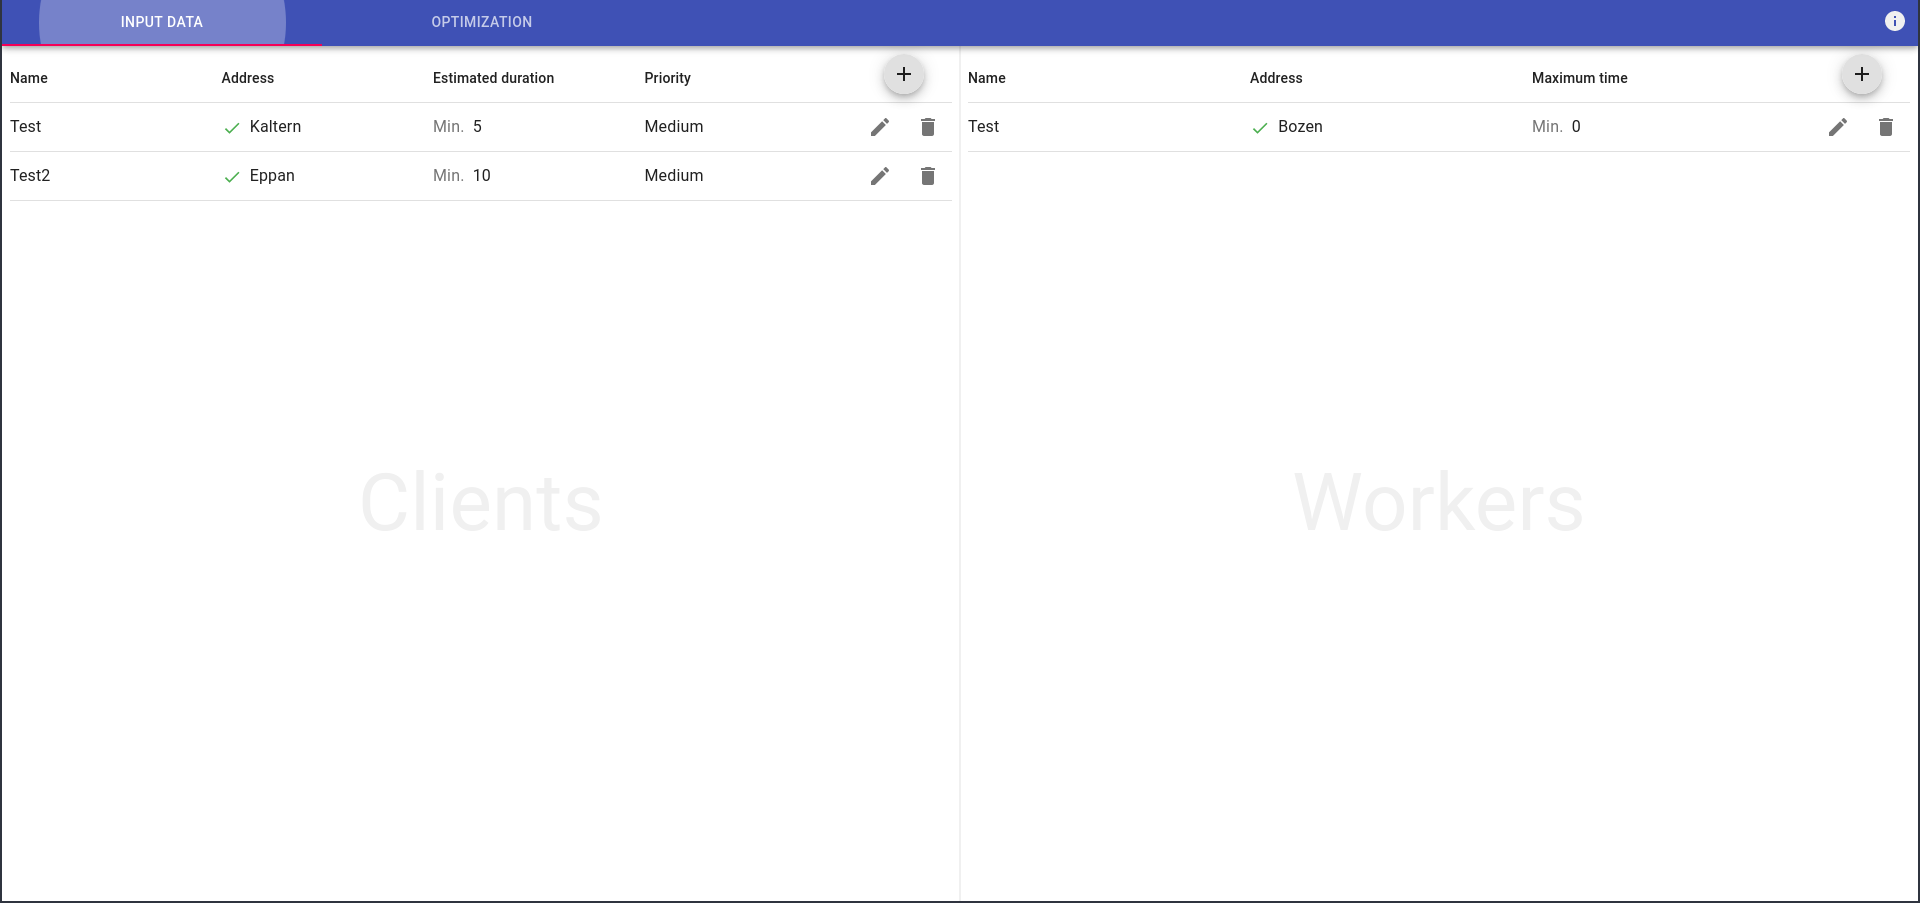
\includegraphics[width=\linewidth]{website-input.png}
        \caption{Dateneingabe Tab}
        \label{fig:websiteData}
    \end{subfigure}
    \begin{subfigure}[b]{0.75\linewidth}
        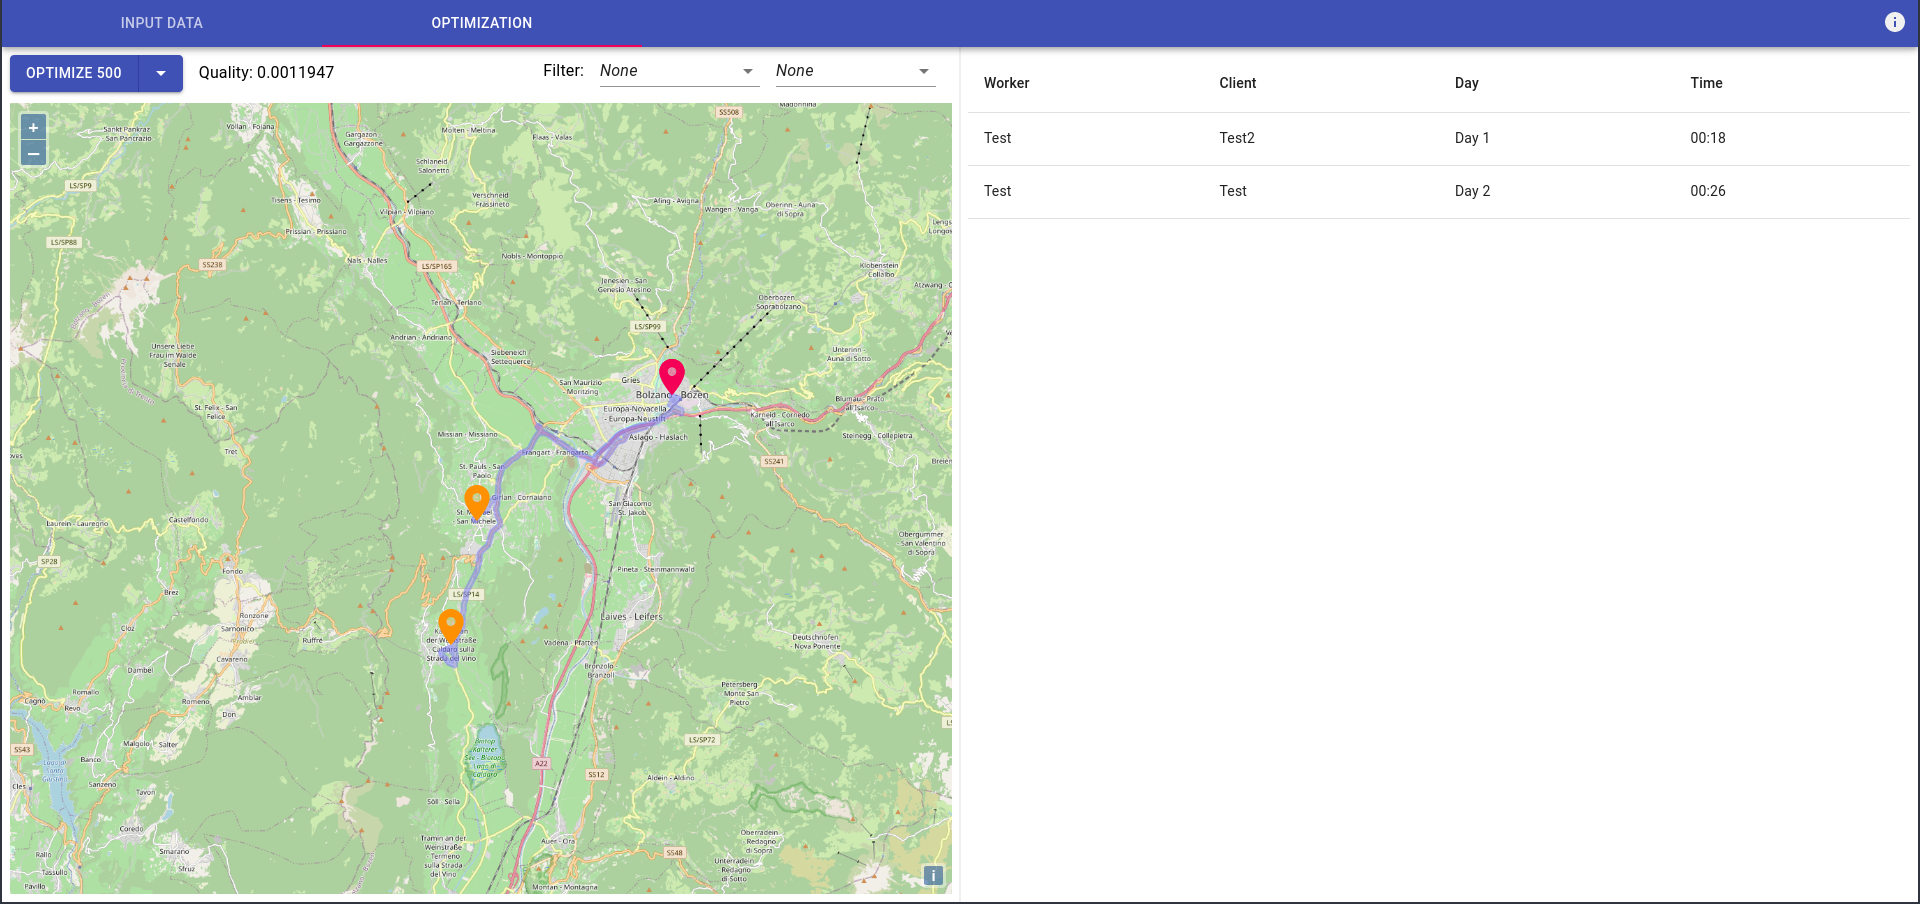
\includegraphics[width=\linewidth]{website-optimization.png}
        \caption{Optimierungs Tab}
        \label{fig:websiteOptim}
    \end{subfigure}
    \caption{Benutzerinterface der Webanwendung}
    \label{fig:website}
\end{figure}

Die Website besteht aus zwei verschiedenen Tabs. Ein Tab davon wird für
die Eingabe der Daten verwendet (Abbildung \ref{fig:websiteData}), in
welchem man sowohl die Einsätze als auch die Techniker eintragen kann
und alle benötigten Parameter einstellen kann.

Der zweite Tab (Abbildung \ref{fig:websiteOptim}) kann nur dann geöffnet
werden, wenn die benötigten Daten eingetragen
wurden und dient zum Errechnen und Anzeigen der optimierten Lösung. Um
die Lösung zu optimieren, kann der „Optimize“-Knopf genutzt werden. Man kann
bei diesem Knopf auch einstellen wie viele Iterationen durchgeführt werden
sollen und nach der Optimierung, wird die Tabelle und Karte aktualisiert.

\chapter{Schluss}

\section{Einschränkungen}

Der Algorithmus wird bei größeren Eingaben natürlicherweise immer langsamer
und es wird auch immer schwieriger die optimale Lösung zu finden. Auch
sind die Einstellungsmöglichkeiten relativ eingeschränkt, aber man könnte
relativ einfach weitere Kriterien zum Algorithmus hinzuzufügen, da ich
mich für eine Metaheuristik entschieden habe. Das heißt aber auch, dass
bei einer gewissen Größe es nicht mehr möglich ist die optimale Lösung
zu erwarten.

\section{Erweiterungsmöglichkeiten}

Der Algorithmus kann noch optimiert werden. So können zum Beispiel noch
weitere Kriterien für eine Lösung hinzugefügt werden, wie zum Beispiel
ein Fenster, innerhalb welchem ein Einsatz ausgeführt werden muss.
Auch die internen Parameter der Algorithmus, wie die Mutationsrate
oder die Populationsgröße, könnten vielleicht noch feiner eingestellt
werden, um eine schnellere Konvergenz zu ermöglichen.

\newpage
\addcontentsline{toc}{chapter}{Literaturverzeichnis}
\nocite{*}
\bibliography{report}
\bibliographystyle{ieeetr}

\end{document}
